\documentclass[12pt, a4paper]{article}

%%%%% Packages

\usepackage{verbatim}
\usepackage[width=18.8cm, left=1.1cm, height=25.9cm, top=1.7cm]{geometry}
\usepackage{amsmath,graphicx}
\usepackage{amssymb, amsthm}
\usepackage{color, enumitem}
\usepackage{arcs} %\overarc{...} arc of circle
\usepackage{pifont}
\usepackage{soul}
\usepackage{wrapfig}
\usepackage{fancybox}
\usepackage{harpoon}
\usepackage{pgfplots}
\usepackage{tikz}
\usetikzlibrary{positioning}
\usetikzlibrary{shapes.multipart}
\usepackage{fancyhdr}
\pagestyle{fancy}
\renewcommand{\familydefault}{\rmdefault}
\usepackage{multicol}
\setlength{\parindent}{0cm}
\usepackage{fontspec} %加這個就可以設定字體
\usepackage{fourier}
\usepackage{cleveref}
\usepackage[most]{tcolorbox}
\usepackage{lipsum}
\usepackage[framemethod=TikZ]{mdframed}
\usepackage[hidelinks,hypertexnames=false]{hyperref}
\usepackage{xparse}
\usepackage{titlesec}
\usepackage{mathtools}


%%%%% Header and Footer

\renewcommand{\headrulewidth}{0pt}
\rhead{}

\cfoot{P. \thepage}

%%%%% Sbullet

\newcommand\sbullet[1][1]{\mathbin{\vcenter{\hbox{\scalebox{#1}{$\bullet$}}}}}


%%%%% Section Style

\titleformat{\section}
{\bf\LARGE}{\thesection.}{0.3em}{}


%%%%% MathsChris

\renewcommand{\MathsChris}{MathsChris\null}


%%%%% Recurring Decimals


\ExplSyntaxOn

%% Dots on the first and last digit
\NewDocumentCommand{\periodfl}{m}
{
  \repdec_initial_final_dots:n { #1 }
}

\seq_new:N \l__repdec_digits_seq
\tl_new:N \l__repdec_first_tl
\tl_new:N \l__repdec_last_tl

\cs_new_protected:Npn \repdec_initial_final_dots:n #1
{
  \seq_set_split:Nnn \l__repdec_digits_seq {} { #1 }
  \seq_pop_left:NN \l__repdec_digits_seq \l__repdec_first_tl
  \seq_pop_right:NN \l__repdec_digits_seq \l__repdec_last_tl
  \quark_if_no_value:VF \l__repdec_first_tl { \dot{\l__repdec_first_tl} }
  \seq_use:Nnnn \l__repdec_digits_seq {}{}{}
  \quark_if_no_value:VF \l__repdec_last_tl { \dot{\l__repdec_last_tl} }
}
\cs_generate_variant:Nn \quark_if_no_value:nF { V }

%% Dots on all digits
\NewDocumentCommand{\periodalldots}{m}
{
  \repdec_initial_all_dots:n { #1 }
}

\cs_new_protected:Npn \repdec_initial_all_dots:n #1
{
  \tl_map_inline:nn { #1 } { \dot{##1} }
}

%% Bar over period
\NewDocumentCommand{\periodbar}{m}
{
  \overline{ #1 }
}

%% Parentheses around period
\NewDocumentCommand{\periodparens}{m}
{
  (#1)
}

%% Dot on unique digit, bar on several digits
\NewDocumentCommand{\periodmixed}{m}
{
  \repdec_mixed:n { #1 }
}
\cs_new_protected:Npn \repdec_mixed:n #1
{
  \int_case:nnn { \tl_count:n { #1 } }
  {
    { 0 } { }
      { 1 } { \dot{#1} }
  }
  {
    \overline{#1}
  }
}

\ExplSyntaxOff

%%%%%






%%%%% enumitem setting
\setlistdepth{9}
\newlist{enumprob}{enumerate}{9}
\setenumerate[enumprob]{leftmargin=8mm,rightmargin=0pt,label=\arabic*.,labelwidth=8mm, itemsep=6mm, topsep=0mm, labelsep=2mm, labelindent=0pt, align=left, partopsep=5mm}
\setlist[enumprob,1]{label=\arabic*.,widest=999,itemindent=0pt,labelsep=2mm,labelwidth=6mm}
\setlist[enumprob,2]{label=(\alph*)}
\setlist[enumprob,3]{label=(\roman*)}
\setlist[enumprob,4]{label=(\arabic*)}
\setlist[enumprob,5]{label=(\arabic*)}
\setlist[enumprob,6]{label=(\arabic*)}
\setlist[enumprob,7]{label=(\arabic*)}
\setlist[enumprob,8]{label=(\arabic*)}
\setlist[enumprob,9]{label=(\arabic*)}



\setlistdepth{9}
\newlist{enumx}{enumerate}{9}
\setenumerate[enumx]{leftmargin=0.8cm,rightmargin=0pt,label=\arabic*.,labelwidth=6mm, itemsep=3pt, topsep=3mm, labelsep=2mm, labelindent=0pt, align=left, partopsep=0mm}
\setlist[enumx,1]{label=\arabic*.}
\setlist[enumx,2]{label=(\alph*),itemsep=0pt,topsep=0pt}
\setlist[enumx,3]{label=(\roman*)}
\setlist[enumx,4]{label=(\arabic*)}
\setlist[enumx,5]{label=(\arabic*)}
\setlist[enumx,6]{label=(\arabic*)}
\setlist[enumx,7]{label=(\arabic*)}
\setlist[enumx,8]{label=(\arabic*)}
\setlist[enumx,9]{label=(\arabic*)}


\setlistdepth{9}
\newlist{thinkitem}{enumerate}{9}
\setenumerate[thinkitem]{leftmargin=1.2em,rightmargin=0pt,label=\textcolor{green!80!black}{\sbullet[1.5]},itemsep=0pt,topsep=3pt}

\newlist{itemlist}{enumerate}{9}
\setenumerate[itemlist]{leftmargin=1.2em,rightmargin=0pt,label={\sbullet[1.5]},itemsep=0pt,topsep=3pt}

\setlistdepth{9}
\newlist{planitem}{enumerate}{9}
\setenumerate[planitem]{leftmargin=*,rightmargin=0pt,label=\arabic*.,itemsep=0pt,topsep=3pt,widest=99}
\setlist[planitem,1]{label=\arabic*.}
\setlist[planitem,2]{label=(\alph*)}
\setlist[planitem,3]{label=(\roman*)}
\setlist[planitem,4]{label=(\arabic*)}
\setlist[planitem,5]{label=(\arabic*)}
\setlist[planitem,6]{label=(\arabic*)}
\setlist[planitem,7]{label=(\arabic*)}
\setlist[planitem,8]{label=(\arabic*)}
\setlist[planitem,9]{label=(\arabic*)}

\newlist{steps}{enumerate}{9}
\setenumerate[steps]{leftmargin=*,rightmargin=0pt,label=Step~\arabic*.,itemsep=0pt,topsep=3pt,widest=99}
\setlist[steps,1]{label=Step \arabic*.}
\setlist[steps,2]{label=(\alph*)}
\setlist[steps,3]{label=(\roman*)}
\setlist[steps,4]{label=(\arabic*)}
\setlist[steps,5]{label=(\arabic*)}
\setlist[steps,6]{label=(\arabic*)}
\setlist[steps,7]{label=(\arabic*)}
\setlist[steps,8]{label=(\arabic*)}
\setlist[steps,9]{label=(\arabic*)}

\newlist{writesteps}{enumerate}{9}
\setenumerate[writesteps]{leftmargin=*,rightmargin=0pt,label={\small \tt \textcolor{blue}{\arabic*.}},itemsep=0pt,topsep=3pt,widest=99}
\setlist[writesteps,1]{label={\small \tt \textcolor{blue}{\arabic*.}}}
\setlist[writesteps,2]{label={\small \tt \textcolor{blue}{(\alph*)}}}
\setlist[writesteps,3]{label=(\roman*)}
\setlist[writesteps,4]{label=(\arabic*)}
\setlist[writesteps,5]{label=(\arabic*)}
\setlist[writesteps,6]{label=(\arabic*)}
\setlist[writesteps,7]{label=(\arabic*)}
\setlist[writesteps,8]{label=(\arabic*)}
\setlist[writesteps,9]{label=(\arabic*)}

\newcommand{\planstep}[1]{\ensuremath{\text{\small \tt \textcolor{blue}{[#1]}}}}




%%%%% Fonts Setting
\setmainfont{Times New Roman}
\usepackage{xeCJK}  %讓中英文字體分開設置
\setCJKmainfont{新細明體} %設定中文為系統上的字型,而英文不去更動,使用原TeX字%型
\XeTeXlinebreaklocale "zh"   %這兩行一定要加,中文才能自動換行
\XeTeXlinebreakskip = 0pt plus 1pt %這兩行一定要加,中文才能自動換行

%%%%% User Defined Functions
\newcommand{\abs}[1]{\left|#1\right|}
\newcommand{\dps}{\displaystyle}
\newcommand{\parallelsum}{\mathbin{\!/\mkern-5mu/\!}}
\renewcommand{\overarc}[1]{\widearc{#1}}
\newcommand{\any}{\forall\, }
\newcommand{\degree}{\ensuremath{^{\circ}}}
\renewcommand{\d}{\mbox{d}}

\newcommand{\NF}{
  \begin{tikzpicture}
    \node[inner sep=0.1cm, preaction={fill=black,fill opacity=0.15},rounded corners=0.1ex,font=\fontsize{7pt}{17pt}\selectfont] (c) {\textbf{NF}}
  \end{tikzpicture}
}

%%% Vectors
\renewcommand{\i}{\mathbf{i}}
\renewcommand{\j}{\mathbf{j}}
\renewcommand{\k}{\mathbf{k}}
\renewcommand{\vec}[1]{\overrightharp{#1}}

%%%%% Marking Style
\renewcommand{\marks}[1]{\hfill\null\hfill (#1~marks)}
\newcommand{\onemark}{\hfill\null\hfill (1~mark)}

%%%%% Graphics

\newcommand{\graphics}[1]{\par
  \begin{center}
    \includegraphics{#1}
  \end{center}
}

\graphicspath{{D:/DSEbyTopic/Graphics/}}

\newcommand{\mcgraphics}[2]{
  \null\par
  \vspace{-3mm}
  \begin{minipage}[t]{0.45\textwidth}

    #2

  \end{minipage}
  \begin{minipage}[t]{0.5\textwidth}
    \null\par
    \vspace{-0.02\textwidth}

    \begin{flushright}
      \includegraphics{#1}
    \end{flushright}
  \end{minipage}
  \vspace{0.01\textwidth}
}


%%%%% Environments

\newenvironment{absolutelynopagebreak}
{\nobreak\vfil\penalty0\vfilneg
  \vtop\bgroup}
{\par\xdef\tpd{\the\prevdepth}\egroup
  \prevdepth=\tpd}

\newcommand{\greybox}[1]{
  \begin{tikzpicture}
    \node[inner sep=0.3cm, preaction={fill=black,fill opacity=0.15},rounded corners=1ex,font=\fontsize{24pt}{24pt}\selectfont] (c) {#1}
  \end{tikzpicture}
}

\SetLabelAlign{parright}{\parbox[t]{\labelwidth}{\raggedleft‌​#1}}


%%%%% get and put

\newcommand{\sectiontitle}[3]{\input{"D:/DSEbyTopic/SectionTitle/Title_#1_#2_#3.tex"}}


\newcommand{\problem}[2][]{
  \begin{minipage}[t]{(\textwidth-1cm)}
    \input{"D:/DSEbyTopic/Problems/#2.tex"}%
    \ifstrempty{#1}%
    {
    }%
    {\linebreak\null\hfill[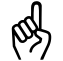
\includegraphics{uppointing}#2]
    }%
  \end{minipage}
}



\newcommand{\problemans}[1]{
  \begin{minipage}[t]{(\textwidth-1cm)}
    \input{"D:/DSEbyTopic/Problems/#1-ans.tex"}
  \end{minipage}
}


%%%%% Graphics


\newcommand{\starr}{
\includegraphics{star}}

\graphicspath{{D:/DSEbyTopic/Graphics/}}

\newcommand{\mcgraphics}[2]{
  \par
  \vspace{0.0001\textwidth}
  \begin{minipage}[t]{0.33\textwidth}

    #2

  \end{minipage}
  \begin{minipage}[t]{0.65\textwidth}
    \null\par
    \vspace{-0.12\textwidth}

    \begin{flushright}
      \includegraphics{#1}
    \end{flushright}
  \end{minipage}
  \vspace{0.01\textwidth}
}



%%%%% environment commands


%%%%% TC environment

\newcounter{tccounter}
\setcounter{tccounter}{0}
\renewcommand{\thetccount}{\arabic{tccounter}}
\newenvironment{theorem}[2][]{%
  \refstepcounter{tccounter}%
  \ifstrempty{#1}%
  {\mdfsetup{%
      frametitle={%
          \tikz[baseline=(current bounding box.east),outer sep=0pt]
          \node[anchor=east,rectangle,fill=blue!20]
          {\strut Theorem~\thetccount};}}
  }%
  {\mdfsetup{%
      frametitle={%
          \tikz[baseline=(current bounding box.east),outer sep=0pt]
          \node[anchor=east,rectangle,fill=blue!20]
          {\strut Theorem~\thetccount~(#1)~};}}%
  }%
  \mdfsetup{innertopmargin=4pt,innerbottommargin=10pt,linecolor=blue!20,%
    linewidth=2pt,topline=true,%
    frametitleaboveskip=\dimexpr-\ht\strutbox\relax
  }
  \begin{mdframed}[]\relax%
    \label{#2}}{\end{mdframed}}

\newenvironment{concept}[2][]{%
  \refstepcounter{tccounter}%
  \ifstrempty{#1}%
  {\mdfsetup{%
      frametitle={%
          \tikz[baseline=(current bounding box.east),outer sep=0pt]
          \node[anchor=east,rectangle,fill=blue!20]
          {\strut Concept~\thetccount};}}
  }%
  {\mdfsetup{%
      frametitle={%
          \tikz[baseline=(current bounding box.east),outer sep=0pt]
          \node[anchor=east,rectangle,fill=blue!20]
          {\strut Concept~\thetccount~(#1)~};}}%
  }%
  \mdfsetup{innertopmargin=4pt,innerbottommargin=10pt,linecolor=blue!20,%
    linewidth=2pt,topline=true,%
    frametitleaboveskip=\dimexpr-\ht\strutbox\relax
  }
  \begin{mdframed}[]\relax%
    \label{#2}}{\end{mdframed}}

\newenvironment{formula}[2][]{%
  \refstepcounter{tccounter}%
  \ifstrempty{#1}%
  {\mdfsetup{%
      frametitle={%
          \tikz[baseline=(current bounding box.east),outer sep=0pt]
          \node[anchor=east,rectangle,fill=blue!20]
          {\strut Formula~\thetccount};}}
  }%
  {\mdfsetup{%
      frametitle={%
          \tikz[baseline=(current bounding box.east),outer sep=0pt]
          \node[anchor=east,rectangle,fill=blue!20]
          {\strut Formula~\thetccount~(#1)~};}}%
  }%
  \mdfsetup{innertopmargin=4pt,innerbottommargin=10pt,linecolor=blue!20,%
    linewidth=2pt,topline=true,%
    frametitleaboveskip=\dimexpr-\ht\strutbox\relax
  }
  \begin{mdframed}[]\relax%
    \label{#2}}{\end{mdframed}}


\newenvironment{presentation}[2][]{%
  \refstepcounter{tccounter}%
  \ifstrempty{#1}%
  {\mdfsetup{%
      frametitle={%
          \tikz[baseline=(current bounding box.east),outer sep=0pt]
          \node[anchor=east,rectangle,fill=blue!20]
          {\strut Presentation~\thetccount};}}
  }%
  {\mdfsetup{%
      frametitle={%
          \tikz[baseline=(current bounding box.east),outer sep=0pt]
          \node[anchor=east,rectangle,fill=blue!20]
          {\strut Presentation~\thetccount~(#1)~};}}%
  }%
  \mdfsetup{innertopmargin=4pt,innerbottommargin=10pt,linecolor=blue!20,%
    linewidth=2pt,topline=true,%
    frametitleaboveskip=\dimexpr-\ht\strutbox\relax
  }
  \begin{mdframed}[]\relax%
    \label{#2}}{\end{mdframed}}


%%%%% LP environment

\newcounter{lpcounter}
\setcounter{lpcounter}{0}
\renewcommand{\thelpcount}{\arabic{lpcounter}}

\newenvironment{skill}[2][]{%
  \refstepcounter{lpcounter}%
  \ifstrempty{#1}%
  {\mdfsetup{%
      frametitle={%
          \tikz[baseline=(current bounding box.east),outer sep=0pt]
          \node[anchor=east,rectangle,fill=red!20]
          {\strut Skill~\thelpcount};}}
  }%
  {\mdfsetup{%
      frametitle={%
          \tikz[baseline=(current bounding box.east),outer sep=0pt]
          \node[anchor=east,rectangle,fill=red!20]
          {\strut Skill~\thelpcount~(#1)~};}}%
  }%
  \mdfsetup{innertopmargin=4pt,innerbottommargin=10pt,linecolor=red!20,%
    linewidth=2pt,topline=true,%
    frametitleaboveskip=\dimexpr-\ht\strutbox\relax
  }
  \begin{mdframed}[]\relax%
    \label{#2}}{\end{mdframed}}


\newenvironment{trick}[2][]{%
  \refstepcounter{lpcounter}%
  \ifstrempty{#1}%
  {\mdfsetup{%
      frametitle={%
          \tikz[baseline=(current bounding box.east),outer sep=0pt]
          \node[anchor=east,rectangle,fill=red!20]
          {\strut Trick~\thelpcount};}}
  }%
  {\mdfsetup{%
      frametitle={%
          \tikz[baseline=(current bounding box.east),outer sep=0pt]
          \node[anchor=east,rectangle,fill=red!20]
          {\strut Trick~\thelpcount~(#1)~};}}%
  }%
  \mdfsetup{innertopmargin=4pt,innerbottommargin=10pt,linecolor=red!20,%
    linewidth=2pt,topline=true,%
    frametitleaboveskip=\dimexpr-\ht\strutbox\relax
  }
  \begin{mdframed}[]\relax%
    \label{#2}}{\end{mdframed}}


\newenvironment{fact}[2][]{%
  \refstepcounter{lpcounter}%
  \ifstrempty{#1}%
  {\mdfsetup{%
      frametitle={%
          \tikz[baseline=(current bounding box.east),outer sep=0pt]
          \node[anchor=east,rectangle,fill=red!20]
          {\strut Fact~\thelpcount};}}
  }%
  {\mdfsetup{%
      frametitle={%
          \tikz[baseline=(current bounding box.east),outer sep=0pt]
          \node[anchor=east,rectangle,fill=red!20]
          {\strut Fact~\thelpcount~(#1)~};}}%
  }%
  \mdfsetup{innertopmargin=4pt,innerbottommargin=10pt,linecolor=red!20,%
    linewidth=2pt,topline=true,%
    frametitleaboveskip=\dimexpr-\ht\strutbox\relax
  }
  \begin{mdframed}[]\relax%
    \label{#2}}{\end{mdframed}}


\newenvironment{skillgroup}[2][]{%
  \refstepcounter{lpcounter}%
  \ifstrempty{#1}%
  {\mdfsetup{%
      frametitle={%
          \tikz[baseline=(current bounding box.east),outer sep=0pt]
          \node[anchor=east,rectangle,fill=red!20]
          {\strut Skill Group~\thelpcount};}}
  }%
  {\mdfsetup{%
      frametitle={%
          \tikz[baseline=(current bounding box.east),outer sep=0pt]
          \node[anchor=east,rectangle,fill=red!20]
          {\strut Skill Group~\thelpcount~(#1)~};}}%
  }%
  \mdfsetup{innertopmargin=4pt,innerbottommargin=10pt,linecolor=red!20,%
    linewidth=2pt,topline=true,%
    frametitleaboveskip=\dimexpr-\ht\strutbox\relax
  }
  \begin{mdframed}[]\relax%
    \label{#2}}{\end{mdframed}}


\newenvironment{trickgroup}[2][]{%
  \refstepcounter{lpcounter}%
  \ifstrempty{#1}%
  {\mdfsetup{%
      frametitle={%
          \tikz[baseline=(current bounding box.east),outer sep=0pt]
          \node[anchor=east,rectangle,fill=red!20]
          {\strut Trick Group~\thelpcount};}}
  }%
  {\mdfsetup{%
      frametitle={%
          \tikz[baseline=(current bounding box.east),outer sep=0pt]
          \node[anchor=east,rectangle,fill=red!20]
          {\strut Trick Group~\thelpcount~(#1)~};}}%
  }%
  \mdfsetup{innertopmargin=4pt,innerbottommargin=10pt,linecolor=red!20,%
    linewidth=2pt,topline=true,%
    frametitleaboveskip=\dimexpr-\ht\strutbox\relax
  }
  \begin{mdframed}[]\relax%
    \label{#2}}{\end{mdframed}}


\newenvironment{factgroup}[2][]{%
  \refstepcounter{lpcounter}%
  \ifstrempty{#1}%
  {\mdfsetup{%
      frametitle={%
          \tikz[baseline=(current bounding box.east),outer sep=0pt]
          \node[anchor=east,rectangle,fill=red!20]
          {\strut Fact Group~\thelpcount};}}
  }%
  {\mdfsetup{%
      frametitle={%
          \tikz[baseline=(current bounding box.east),outer sep=0pt]
          \node[anchor=east,rectangle,fill=red!20]
          {\strut Fact Group~\thelpcount~(#1)~};}}%
  }%
  \mdfsetup{innertopmargin=4pt,innerbottommargin=10pt,linecolor=red!20,%
    linewidth=2pt,topline=true,%
    frametitleaboveskip=\dimexpr-\ht\strutbox\relax
  }
  \begin{mdframed}[]\relax%
    \label{#2}}{\end{mdframed}}

\newenvironment{pattern}[2][]{%
  \refstepcounter{lpcounter}%
  \ifstrempty{#1}%
  {\mdfsetup{%
      frametitle={%
          \tikz[baseline=(current bounding box.east),outer sep=0pt]
          \node[anchor=east,rectangle,fill=red!20]
          {\strut Pattern~\thelpcount};}}
  }%
  {\mdfsetup{%
      frametitle={%
          \tikz[baseline=(current bounding box.east),outer sep=0pt]
          \node[anchor=east,rectangle,fill=red!20]
          {\strut Pattern~\thelpcount~(#1)~};}}%
  }%
  \mdfsetup{innertopmargin=4pt,innerbottommargin=10pt,linecolor=red!20,%
    linewidth=2pt,topline=true,%
    frametitleaboveskip=\dimexpr-\ht\strutbox\relax
  }
  \begin{mdframed}[]\relax%
    \label{#2}}{\end{mdframed}}


\newcounter{illucounter}[lpcounter]
\setcounter{illucounter}{0}
\renewcommand{\theillucounter}{\thelpcounter.\arabic{illucounter}}

\newenvironment{illustration}[2][]{%
  \refstepcounter{illucounter}%
  \ifstrempty{#1}%
  {\mdfsetup{%
      frametitle={%
          \tikz[baseline=(current bounding box.east),outer sep=0pt]
          \node[anchor=east,rectangle,fill=red!10]
          {\strut Illustration~\theillucounter};}}
  }%
  {\mdfsetup{%
      frametitle={%
          \tikz[baseline=(current bounding box.east),outer sep=0pt]
          \node[anchor=east,rectangle,fill=red!10]
          {\strut Illustration~\theillucounter~(#1)~};}}%
  }%
  \mdfsetup{innertopmargin=4pt,innerbottommargin=10pt,linecolor=red!10,%
    linewidth=2pt,topline=true,%
    frametitleaboveskip=\dimexpr-\ht\strutbox\relax
  }
  \begin{mdframed}[]\relax%
    \label{#2}}{\end{mdframed}}

\newenvironment{tiy}[2][]{%
  \refstepcounter{illucounter}%
  \ifstrempty{#1}%
  {\mdfsetup{%
      frametitle={%
          \tikz[baseline=(current bounding box.east),outer sep=0pt]
          \node[anchor=east,rectangle,fill=red!20]
          {\strut Try it Yourself~\theillucounter};}}
  }%
  {\mdfsetup{%
      frametitle={%
          \tikz[baseline=(current bounding box.east),outer sep=0pt]
          \node[anchor=east,rectangle,fill=red!20]
          {\strut Try it Yourself~\theillucounter~(#1)~};}}%
  }%
  \mdfsetup{innertopmargin=4pt,innerbottommargin=10pt,linecolor=red!20,%
    linewidth=2pt,topline=true,%
    frametitleaboveskip=\dimexpr-\ht\strutbox\relax
  }
  \begin{mdframed}[]\relax%
    \label{#2}}{\end{mdframed}}



%%%%% Eg Environments

\newcounter{egcounter}
\setcounter{egcounter}{0}
\renewcommand{\theegcount}{\arabic{egcounter}}
\newenvironment{example}[2][]{%
  \begin{absolutelynopagebreak}
    \refstepcounter{egcounter}%
    \ifstrempty{#1}%
    {\mdfsetup{%
        frametitle={%
            \tikz[baseline=(current bounding box.east),outer sep=0pt]
            \node[anchor=east,rectangle,fill=green!40]
            {\strut Example~\theegcount};}}
    }%
    {\mdfsetup{%
        frametitle={%
            \tikz[baseline=(current bounding box.east),outer sep=0pt]
            \node[anchor=east,rectangle,fill=green!40]
            {\strut Example~\theegcount~(#1)~};}}%
    }%
    \mdfsetup{innertopmargin=4pt,innerbottommargin=10pt,linecolor=green!40,%
      linewidth=2pt,topline=true,%
      frametitleaboveskip=\dimexpr-\ht\strutbox\relax,
      skipabove=0pt,skipbelow=25pt,
    }
    \begin{mdframed}[]\relax%
      \label{#2}}{\end{mdframed}\end{absolutelynopagebreak}}


\newenvironment{Question}[2][]{%
  \begin{absolutelynopagebreak}
    \refstepcounter{egcounter}%
    \ifstrempty{#1}%
    {\mdfsetup{%
        frametitle={%
            \tikz[baseline=(current bounding box.east),outer sep=0pt]
            \node[anchor=east,rectangle,fill=green!40]
            {\strut Example~\ref{#2}};}}
    }%
    {\mdfsetup{%
        frametitle={%
            \tikz[baseline=(current bounding box.east),outer sep=0pt]
            \node[anchor=east,rectangle,fill=green!40]
            {\strut Example~\ref{#2}~(#1)~};}}%
    }%
    \mdfsetup{innertopmargin=4pt,innerbottommargin=10pt,linecolor=green!40,%
      linewidth=2pt,topline=true,%
      frametitleaboveskip=\dimexpr-\ht\strutbox\relax,
      skipabove=0pt,skipbelow=25pt,
    }
    \begin{mdframed}[]\relax%
      }{\end{mdframed}\end{absolutelynopagebreak}}






\newenvironment{Read}{%
  \begin{mdframed}[%
      frametitle={
\includegraphics{Read}~Read the Question},
      apptotikzsetting={\tikzset{mdfframetitlebackground/.append style={%
              shade,left color=green!20!white, right color=white}}},
      %frametitlerule=true,
      %frametitlerulewidth=1pt,
      %frametitlerulecolor=black,
      innertopmargin=0.7em,%
      innerleftmargin=0.7em,%,
      innerrightmargin=0.7em,
      hidealllines=true,leftline=true,
      frametitlebackgroundcolor=green!20,
      linewidth=3pt,
      linecolor=green!20,
      skipabove=0pt,skipbelow=0pt,
      %fontcolor=white,%
      %backgroundcolor=green!10
    ]%
    }{%
  \end{mdframed}
}

\newcommand{\readrule}{\textcolor{green!80!black}{\hrulefill}}
\newcommand{\illustrationrule}{\textcolor{red!10}{\hrulefill}}



\newenvironment{Think}{%
  \begin{mdframed}[%
      frametitle={
\includegraphics{Think}~Thinking Process},
      apptotikzsetting={\tikzset{mdfframetitlebackground/.append style={%
              shade,left color=green!20!white, right color=white}}},
      %frametitlerule=true,
      %frametitlerulewidth=1pt,
      %frametitlerulecolor=black,
      innertopmargin=0.7em,%
      innerleftmargin=0.7em,%,
      innerrightmargin=0.7em,
      hidealllines=true,leftline=true,
      frametitlebackgroundcolor=green!20,
      linewidth=3pt,
      linecolor=green!20,
      skipabove=0pt,skipbelow=0pt,
      %fontcolor=white,%
      %backgroundcolor=green!10
    ]%
    }{%
  \end{mdframed}
}

\newenvironment{Plan}{%
  \begin{mdframed}[%
      frametitle={
\includegraphics{Plan}~Plan of Attack},
      apptotikzsetting={\tikzset{mdfframetitlebackground/.append style={%
              shade,left color=green!20!white, right color=white}}},
      %frametitlerule=true,
      %frametitlerulewidth=1pt,
      %frametitlerulecolor=black,
      innertopmargin=0.7em,%
      innerleftmargin=0.7em,%,
      innerrightmargin=0.7em,
      hidealllines=true,leftline=true,
      frametitlebackgroundcolor=green!20,
      linewidth=3pt,
      linecolor=green!20,
      skipabove=0pt,skipbelow=0pt,
      %fontcolor=white,%
      %backgroundcolor=green!10
    ]%
    }{%
  \end{mdframed}
}

\newenvironment{Remark}{%
  \begin{mdframed}[%
      frametitle={Remarks and Comments},
      apptotikzsetting={\tikzset{mdfframetitlebackground/.append style={%
              shade,left color=green!20!white, right color=white}}},
      %frametitlerule=true,
      %frametitlerulewidth=1pt,
      %frametitlerulecolor=black,
      innertopmargin=0.7em,%
      innerleftmargin=0.7em,%,
      innerrightmargin=0.7em,
      hidealllines=true,leftline=true,
      frametitlebackgroundcolor=green!20,
      linewidth=3pt,
      linecolor=green!20,
      skipabove=0pt,skipbelow=0pt,
      %fontcolor=white,%
      %backgroundcolor=green!10
    ]%
    }{%
  \end{mdframed}
}

\newenvironment{Write}{%
  \begin{mdframed}[%
      frametitle={
\includegraphics{Write}~What to Write},
      apptotikzsetting={\tikzset{mdfframetitlebackground/.append style={%
              shade,left color=green!30!white, right color=white}}},
      %frametitlerule=true,
      %frametitlerulewidth=1pt,
      %frametitlerulecolor=black,
      innertopmargin=0.7em,%
      innerleftmargin=0.7em,%,
      innerrightmargin=0.7em,
      hidealllines=true,leftline=true, bottomline=true,
      frametitlebackgroundcolor=green!30,
      linewidth=3pt,
      linecolor=green!30,
      %fontcolor=white,%
      %backgroundcolor=green!10
    ]%
    \large
    }{%
  \end{mdframed}
}






%%%%% highlight box


\newtcbox{\lbox}{enhanced,nobeforeafter,tcbox raise base,boxrule=1.3pt,top=0mm,bottom=0mm,right=0.05mm,left=0.05mm,arc=0pt,boxsep=2pt,before upper={\vphantom{dlg}},
  colframe=green!80!black, colback=white
}


\newtcbox{\dbox}{enhanced,nobeforeafter,tcbox raise base,boxrule=0.7pt,top=0.2mm,bottom=0.1mm,right=0.7mm,left=0.7mm,arc=0pt,boxsep=3pt,before upper={\vphantom{\textrm{dlg}}\tt\small},
  colframe=green!80!black, colback=green!80!black, coltext=white
}


\newcommand{\ldbox}[2]{ \lbox{#1}\nolinebreak\dbox{#2} }




\newtcbox{\wbox}{enhanced,nobeforeafter,tcbox raise base,boxrule=0.7pt,top=0.2mm,bottom=0.1mm,right=1.1mm,left=0.7mm,arc=3pt,boxsep=3pt,before upper={\vphantom{dlg}},
  colframe=black,colback=white
}




%%%%% For Reference

\newcommand{\myref}[2]{ \wbox{\hyperref[#2]{#1~\ref{#2}}} }


%%%%% CW MathsNotes

\newcommand{\CWMathsNotes}{\includegraphics[scale=0.6]{CW_MathsNotes}}




%%%%% 

\newcommand{\DSEsectionAone}{\textbf{Paper 1 - A(1)}

}
\newcommand{\DSEsectionAtwo}{\textbf{Paper 1 - A(2)}

}
\newcommand{\DSEsectionB}{\textbf{Paper 1 - B}

}
\newcommand{\DSEMCsectionA}{\textbf{Paper 2 - A}

}
\newcommand{\DSEMCsectionB}{\textbf{Paper 2 - B}

}

\newcommand{\showstat}[1]{#1}


\newcommand{\DSESyl}[1]{

}

\newcommand{\DSETopicName}[1]{

}
\SetLabelAlign{parright}{\parbox[t]{\labelwidth}{\raggedleft‌​#1}}




\usetikzlibrary{shapes,shadows}
\tikzstyle{abstractbox} = [draw=black, fill=white, rectangle,
inner sep=10pt, style=rounded corners, drop shadow={fill=black,
    opacity=0.5}]
\tikzstyle{abstracttitle} =[fill=white]

\newcommand{\sectionsummary}[2][fill=white]{
  \begin{center}
    \begin{tikzpicture}
      \node [abstractbox, #1] (box)
      {\begin{minipage}{0.80\linewidth}
          %            \setlength{\parindent}{2mm}
          \footnotesize #2
        \end{minipage}};
      \node[abstracttitle, right=10pt] at (box.north west) {Section Summary};
    \end{tikzpicture}
  \end{center}
}





\begin{document}
\newpage
\newpage
\thispagestyle{empty}
\rhead{Overview of S6 Chapters}
\lfoot{S6 Chapters}
\begin{center}
Mathematics Revision Notes\\\vspace{1cm}
\greybox{\fontsize{24pt}{24pt}\selectfont {S6 Chapters}} \\\vspace{1cm}
\end{center}
\vspace{0.5cm}
\hline
\section*{Chapter List}
\begin{enumx}[label=Ch \arabic*. , leftmargin=2cm,rightmargin=0pt,labelwidth=17mm, itemsep=3pt, topsep=3mm, labelsep=2mm, labelindent=0pt, align=left, partopsep=0mm ]
\item \hyperref[chapter:S6-1]{Arithmetic and Geometric Sequences} \hfill P.\pageref{chapter:S6-1}
\item \hyperref[chapter:S6-2]{Summation of Arithmetic and Geometric Sequences \NF} \hfill P.\pageref{chapter:S6-2}
\item \hyperref[chapter:S6-3]{More about Graphs of Functions} \hfill P.\pageref{chapter:S6-3}
\item \hyperref[chapter:S6-4]{Uses and Abuses of Statistics} \hfill P.\pageref{chapter:S6-4}
\end{enumx}
\section*{Mark Distribution from Chapter 1 to Chapter 4}
%Graph
\begin{center}
\begin{tikzpicture}
\begin{axis}[
width=18cm,
height=7cm,
bar width=0.6cm,
ybar,
ylabel={Weight},
xticklabels={
Ch 1,Ch 2,Ch 3,Ch 4},
xtick=data,
ymin=0,
nodes near coords,
nodes near coords align={vertical},
x tick label style={rotate=45,anchor=east},
]
\addplot coordinates {(1,56)(2,60)(3,74)(4,1)};
\end{axis}
\end{tikzpicture}
\end{center}



%Graph
\begin{center}
\begin{tikzpicture}
\begin{axis}[
width=18cm,
height=7cm,
bar width=0.6cm,
ybar,
ylabel={P1 Marks},
xticklabels={
Ch 1,Ch 2,Ch 3,Ch 4},
xtick=data,
ymin=0,
nodes near coords,
nodes near coords align={vertical},
x tick label style={rotate=45,anchor=east},
]
\addplot coordinates {(1,46)(2,52)(3,60)(4,0)};
\end{axis}
\end{tikzpicture}
\end{center}



%Graph
\begin{center}
\begin{tikzpicture}
\begin{axis}[
width=18cm,
height=7cm,
bar width=0.6cm,
ybar,
ylabel={P2 Marks},
xticklabels={
Ch 1,Ch 2,Ch 3,Ch 4},
xtick=data,
ymin=0,
nodes near coords,
nodes near coords align={vertical},
x tick label style={rotate=45,anchor=east},
]
\addplot coordinates {(1,10)(2,8)(3,14)(4,1)};
\end{axis}
\end{tikzpicture}
\end{center}



\newpage
\newpage
\thispagestyle{empty}
\rhead{Arithmetic and Geometric Sequences}
\lfoot{S6-Ch1}
\begin{center}
Mathematics Revision Notes\\\vspace{1cm}
\greybox{S6-Ch1}\\\vspace{1cm}
{\fontsize{24pt}{24pt}\selectfont {Arithmetic and Geometric Sequences}} \\\vspace{1cm}
\phantomsection\label{chapter:S6-1}

\end{center}
\vspace{0.5cm}
\hline
\section*{Section List}
\begin{enumx}[label=Sec 1.\arabic*\ ]
\item \hyperref[section:6-1-1]{Review on Sequences}
\item \hyperref[section:6-1-2]{Arithmetic Sequences \NF}
\item \hyperref[section:6-1-3]{Geometric Sequences \NF}
\item \hyperref[section:6-1-4]{Problems Involving  Arithmetic and Geometric  Sequences \NF}
\end{enumx}
\begin{absolutelynopagebreak}
\begin{center}
\textbf{DSE Core Paper 1}
\end{center}
\begin{center}
\begin{tabular}{|l|c|c|c|c|c|c|c|c|c|c|c|c|c|c|c|c|}
\hline
        & Sa & Pr & 12 & 13 & 14 & 15 & 16 & 17 & 18 & 19 & 20 & 21 & 22 & 23 & 24 & 25 \\\hline\hline
Sec 1.1 &  &  &  &  &  &  &  &  &  &  &  &  &  &  &  &  \\\hline
Sec 1.2 &  &  &  &  &  $4$ &  &  &  &  &  &  &  &  &  &  &  \\\hline
Sec 1.3 &  &  &  &  &  &  &  &  &  $5$ &  $6$ &  $5$ &  &  &  &  &  \\\hline
Sec 1.4 &  &  &  &  $13$ &  &  &  $5$ &  &  &  &  &  &  &  $8$ &  &  \\\hline
\end{tabular}
\end{center}
\end{absolutelynopagebreak}
\begin{absolutelynopagebreak}
\begin{center}
\textbf{DSE Core Paper 2}
\end{center}
\begin{center}
\begin{tabular}{|l|c|c|c|c|c|c|c|c|c|c|c|c|c|c|c|c|}
\hline
        & Sa & Pr & 12 & 13 & 14 & 15 & 16 & 17 & 18 & 19 & 20 & 21 & 22 & 23 & 24 & 25 \\\hline\hline
Sec 1.1 &  &  &  &  &  &  &  &  &  &  &  &  &  &  &  &  \\\hline
Sec 1.2 &  $1$ &  &  $1$ &  &  &  &  &  $1$ &  $1$ &  &  $1$ &  &  &  &  &  \\\hline
Sec 1.3 &  &  &  &  &  $1$ &  $1$ &  &  &  &  $1$ &  &  $1$ &  $1$ &  &  &  \\\hline
Sec 1.4 &  &  &  &  &  &  &  &  &  &  &  &  &  &  &  &  \\\hline
\end{tabular}
\end{center}
\end{absolutelynopagebreak}
\begin{absolutelynopagebreak}
\begin{center}
\textbf{DSE Question Table}
\end{center}
\begin{center}
\begin{tabular}{|l|c|c|c|c|}
\hline
        & 1.1 & 1.2 & 1.3 & 1.4 \\\hline
\hline
Paper 1 - A(1)&  &  &  &  \\
\hline
Paper 1 - A(2)&  &  &  &  \\
\hline
Paper 1 - B&  & \hyperref[DSE2014-CoreP1-Q16]{2014-P1-Q16} & \hyperref[DSE2018-CoreP1-Q16]{2018-P1-Q16} & \hyperref[DSE2013-CoreP1-Q19]{2013-P1-Q19} \\
&  &  & \hyperref[DSE2019-CoreP1-Q16]{2019-P1-Q16} & \hyperref[DSE2016-CoreP1-Q17]{2016-P1-Q17} \\
&  &  & \hyperref[DSE2020-CoreP1-Q16]{2020-P1-Q16} & \hyperref[DSE2023-CoreP1-Q18]{2023-P1-Q18} \\
\hline
\hline
Paper 2 - A&  &  &  &  \\
\hline
Paper 2 - B&  & \hyperref[DSE2012S-CoreP2-Q36]{Samp-P2-Q36} & \hyperref[DSE2014-CoreP2-Q37]{2014-P2-Q37} &  \\
&  & \hyperref[DSE2012-CoreP2-Q37]{2012-P2-Q37} & \hyperref[DSE2015-CoreP2-Q37]{2015-P2-Q37} &  \\
&  & \hyperref[DSE2017-CoreP2-Q36]{2017-P2-Q36} & \hyperref[DSE2019-CoreP2-Q36]{2019-P2-Q36} &  \\
&  & \hyperref[DSE2018-CoreP2-Q45]{2018-P2-Q45} & \hyperref[DSE2021-CoreP2-Q36]{2021-P2-Q36} &  \\
&  & \hyperref[DSE2020-CoreP2-Q35]{2020-P2-Q35} & \hyperref[DSE2022-CoreP2-Q37]{2022-P2-Q37} &  \\
\hline
\hline
Cross Topic&  &  &  &  \\
\hline
\end{tabular}
\end{center}
\end{absolutelynopagebreak}




% S6 Ch1 - 1.1 Review on Sequences
\section*{Section 1.1 - Review on Sequences}\phantomsection\label{section:6-1-1}





% S6 Ch1 - 1.2 Arithmetic Sequences \NF
\section*{Section 1.2 - Arithmetic Sequences \NF}\phantomsection\label{section:6-1-2}

\textbf{Paper 1 - B}
\begin{enumx}[label=\arabic*.,start=1]
\phantomsection
\item \phantomsection\label{DSE2014-CoreP1-Q16} \problem[2014-P1-Q16]{DSE2014-CoreP1-Q16}
\end{enumx}
\textbf{Paper 2 - B}
\begin{enumx}[label=\arabic*.,start=2]
\phantomsection
\item \phantomsection\label{DSE2012S-CoreP2-Q36} \problem[Samp-P2-Q36]{DSE2012S-CoreP2-Q36}
\phantomsection
\item \phantomsection\label{DSE2012-CoreP2-Q37} \problem[2012-P2-Q37]{DSE2012-CoreP2-Q37}
\phantomsection
\item \phantomsection\label{DSE2017-CoreP2-Q36} \problem[2017-P2-Q36]{DSE2017-CoreP2-Q36}
\phantomsection
\item \phantomsection\label{DSE2018-CoreP2-Q45} \problem[2018-P2-Q45]{DSE2018-CoreP2-Q45}
\phantomsection
\item \phantomsection\label{DSE2020-CoreP2-Q35} \problem[2020-P2-Q35]{DSE2020-CoreP2-Q35}
\end{enumx}




% S6 Ch1 - 1.3 Geometric Sequences \NF
\section*{Section 1.3 - Geometric Sequences \NF}\phantomsection\label{section:6-1-3}

\textbf{Paper 1 - B}
\begin{enumx}[label=\arabic*.,start=7]
\phantomsection
\item \phantomsection\label{DSE2018-CoreP1-Q16} \problem[2018-P1-Q16]{DSE2018-CoreP1-Q16}
\phantomsection
\item \phantomsection\label{DSE2019-CoreP1-Q16} \problem[2019-P1-Q16]{DSE2019-CoreP1-Q16}
\phantomsection
\item \phantomsection\label{DSE2020-CoreP1-Q16} \problem[2020-P1-Q16]{DSE2020-CoreP1-Q16}
\end{enumx}
\textbf{Paper 2 - B}
\begin{enumx}[label=\arabic*.,start=10]
\phantomsection
\item \phantomsection\label{DSE2014-CoreP2-Q37} \problem[2014-P2-Q37]{DSE2014-CoreP2-Q37}
\phantomsection
\item \phantomsection\label{DSE2015-CoreP2-Q37} \problem[2015-P2-Q37]{DSE2015-CoreP2-Q37}
\phantomsection
\item \phantomsection\label{DSE2019-CoreP2-Q36} \problem[2019-P2-Q36]{DSE2019-CoreP2-Q36}
\phantomsection
\item \phantomsection\label{DSE2021-CoreP2-Q36} \problem[2021-P2-Q36]{DSE2021-CoreP2-Q36}
\phantomsection
\item \phantomsection\label{DSE2022-CoreP2-Q37} \problem[2022-P2-Q37]{DSE2022-CoreP2-Q37}
\end{enumx}




% S6 Ch1 - 1.4 Problems Involving  Arithmetic and Geometric  Sequences \NF
\section*{Section 1.4 - Problems Involving  Arithmetic and Geometric  Sequences \NF}\phantomsection\label{section:6-1-4}

\textbf{Paper 1 - B}
\begin{enumx}[label=\arabic*.,start=15]
\phantomsection
\item \phantomsection\label{DSE2013-CoreP1-Q19} \problem[2013-P1-Q19]{DSE2013-CoreP1-Q19}
\phantomsection
\item \phantomsection\label{DSE2016-CoreP1-Q17} \problem[2016-P1-Q17]{DSE2016-CoreP1-Q17}
\phantomsection
\item \phantomsection\label{DSE2023-CoreP1-Q18} \problem[2023-P1-Q18]{DSE2023-CoreP1-Q18}
\end{enumx}
\section*{Answers}
\begin{enumx}[label=\arabic*.,start=1]
\item \problemans{DSE2014-CoreP1-Q16}
\item \problemans{DSE2012S-CoreP2-Q36}
\item \problemans{DSE2012-CoreP2-Q37}
\item \problemans{DSE2017-CoreP2-Q36}
\item \problemans{DSE2018-CoreP2-Q45}
\item \problemans{DSE2020-CoreP2-Q35}
\item \problemans{DSE2018-CoreP1-Q16}
\item \problemans{DSE2019-CoreP1-Q16}
\item \problemans{DSE2020-CoreP1-Q16}
\item \problemans{DSE2014-CoreP2-Q37}
\item \problemans{DSE2015-CoreP2-Q37}
\item \problemans{DSE2019-CoreP2-Q36}
\item \problemans{DSE2021-CoreP2-Q36}
\item \problemans{DSE2022-CoreP2-Q37}
\item \problemans{DSE2013-CoreP1-Q19}
\item \problemans{DSE2016-CoreP1-Q17}
\item \problemans{DSE2023-CoreP1-Q18}
\end{enumx}
\newpage
\newpage
\thispagestyle{empty}
\rhead{Summation of Arithmetic and Geometric Sequences \NF}
\lfoot{S6-Ch2}
\begin{center}
Mathematics Revision Notes\\\vspace{1cm}
\greybox{S6-Ch2}\\\vspace{1cm}
{\fontsize{24pt}{24pt}\selectfont {Summation of Arithmetic and Geometric Sequences \NF}} \\\vspace{1cm}
\phantomsection\label{chapter:S6-2}

\end{center}
\vspace{0.5cm}
\hline
\section*{Section List}
\begin{enumx}[label=Sec 2.\arabic*\ ]
\item \hyperref[section:6-2-1]{Summation of a Sequence \NF}
\item \hyperref[section:6-2-2]{Summation of an Arithmetic Sequence \NF}
\item \hyperref[section:6-2-3]{Summation of a Geometric Sequence \NF}
\item \hyperref[section:6-2-4]{Applications of the Summation of Arithmetic and Geometric Sequences \NF}
\end{enumx}
\begin{absolutelynopagebreak}
\begin{center}
\textbf{DSE Core Paper 1}
\end{center}
\begin{center}
\begin{tabular}{|l|c|c|c|c|c|c|c|c|c|c|c|c|c|c|c|c|}
\hline
        & Sa & Pr & 12 & 13 & 14 & 15 & 16 & 17 & 18 & 19 & 20 & 21 & 22 & 23 & 24 & 25 \\\hline\hline
Sec 2.1 &  &  &  &  &  &  &  &  &  &  &  &  &  &  &  &  \\\hline
Sec 2.2 &  $4$ &  &  &  &  &  &  &  &  &  &  &  $7$ &  $7$ &  &  &  \\\hline
Sec 2.3 &  &  $12$ &  $13$ &  &  &  &  &  &  &  &  &  &  &  &  &  \\\hline
Sec 2.4 &  &  &  &  &  &  $5$ &  &  $4$ &  &  &  &  &  &  &  &  \\\hline
\end{tabular}
\end{center}
\end{absolutelynopagebreak}
\begin{absolutelynopagebreak}
\begin{center}
\textbf{DSE Core Paper 2}
\end{center}
\begin{center}
\begin{tabular}{|l|c|c|c|c|c|c|c|c|c|c|c|c|c|c|c|c|}
\hline
        & Sa & Pr & 12 & 13 & 14 & 15 & 16 & 17 & 18 & 19 & 20 & 21 & 22 & 23 & 24 & 25 \\\hline\hline
Sec 2.1 &  &  &  &  &  &  &  &  &  &  &  &  &  &  &  &  \\\hline
Sec 2.2 &  &  $1$ &  &  $1$ &  &  &  &  &  $1$ &  &  &  $1$ &  &  &  $1$ &  \\\hline
Sec 2.3 &  &  &  &  &  &  &  $1$ &  &  $1$ &  &  &  &  &  &  &  \\\hline
Sec 2.4 &  &  &  &  &  &  &  &  &  &  &  &  &  &  $1$ &  &  \\\hline
\end{tabular}
\end{center}
\end{absolutelynopagebreak}
\begin{absolutelynopagebreak}
\begin{center}
\textbf{DSE Question Table}
\end{center}
\begin{center}
\begin{tabular}{|l|c|c|c|c|}
\hline
        & 2.1 & 2.2 & 2.3 & 2.4 \\\hline
\hline
Paper 1 - A(1)&  &  &  &  \\
\hline
Paper 1 - A(2)&  &  &  &  \\
\hline
Paper 1 - B&  & \hyperref[DSE2012S-CoreP1-Q15]{Samp-P1-Q15} & \hyperref[DSE2012P-CoreP1-Q19]{Prac-P1-Q19} & \hyperref[DSE2015-CoreP1-Q17]{2015-P1-Q17} \\
&  & \hyperref[DSE2021-CoreP1-Q17]{2021-P1-Q17} & \hyperref[DSE2012-CoreP1-Q19]{2012-P1-Q19} & \hyperref[DSE2017-CoreP1-Q16]{2017-P1-Q16} \\
&  & \hyperref[DSE2022-CoreP1-Q17]{2022-P1-Q17} &  &  \\
\hline
\hline
Paper 2 - A&  &  &  &  \\
\hline
Paper 2 - B&  & \hyperref[DSE2012P-CoreP2-Q35]{Prac-P2-Q35} & \hyperref[DSE2016-CoreP2-Q36]{2016-P2-Q36} & \hyperref[DSE2023-CoreP2-Q36]{2023-P2-Q36} \\
&  & \hyperref[DSE2013-CoreP2-Q38]{2013-P2-Q38} & \hyperref[DSE2018-CoreP2-Q43]{2018-P2-Q43} &  \\
&  & \hyperref[DSE2018-CoreP2-Q35]{2018-P2-Q35} &  &  \\
&  & \hyperref[DSE2021-CoreP2-Q45]{2021-P2-Q45} &  &  \\
&  & \hyperref[DSE2024-CoreP2-Q36]{2024-P2-Q36} &  &  \\
\hline
\hline
Cross Topic&  &  &  &  \\
\hline
\end{tabular}
\end{center}
\end{absolutelynopagebreak}




% S6 Ch2 - 2.1 Summation of a Sequence \NF
\section*{Section 2.1 - Summation of a Sequence \NF}\phantomsection\label{section:6-2-1}





% S6 Ch2 - 2.2 Summation of an Arithmetic Sequence \NF
\section*{Section 2.2 - Summation of an Arithmetic Sequence \NF}\phantomsection\label{section:6-2-2}

\textbf{Paper 1 - B}
\begin{enumx}[label=\arabic*.,start=1]
\phantomsection
\item \phantomsection\label{DSE2012S-CoreP1-Q15} \problem[Samp-P1-Q15]{DSE2012S-CoreP1-Q15}
\phantomsection
\item \phantomsection\label{DSE2021-CoreP1-Q17} \problem[2021-P1-Q17]{DSE2021-CoreP1-Q17}
\phantomsection
\item \phantomsection\label{DSE2022-CoreP1-Q17} \problem[2022-P1-Q17]{DSE2022-CoreP1-Q17}
\end{enumx}
\textbf{Paper 2 - B}
\begin{enumx}[label=\arabic*.,start=4]
\phantomsection
\item \phantomsection\label{DSE2012P-CoreP2-Q35} \problem[Prac-P2-Q35]{DSE2012P-CoreP2-Q35}
\phantomsection
\item \phantomsection\label{DSE2013-CoreP2-Q38} \problem[2013-P2-Q38]{DSE2013-CoreP2-Q38}
\phantomsection
\item \phantomsection\label{DSE2018-CoreP2-Q35} \problem[2018-P2-Q35]{DSE2018-CoreP2-Q35}
\phantomsection
\item \phantomsection\label{DSE2021-CoreP2-Q45} \problem[2021-P2-Q45]{DSE2021-CoreP2-Q45}
\phantomsection
\item \phantomsection\label{DSE2024-CoreP2-Q36} \problem[2024-P2-Q36]{DSE2024-CoreP2-Q36}
\end{enumx}




% S6 Ch2 - 2.3 Summation of a Geometric Sequence \NF
\section*{Section 2.3 - Summation of a Geometric Sequence \NF}\phantomsection\label{section:6-2-3}

\textbf{Paper 1 - B}
\begin{enumx}[label=\arabic*.,start=9]
\phantomsection
\item \phantomsection\label{DSE2012P-CoreP1-Q19} \problem[Prac-P1-Q19]{DSE2012P-CoreP1-Q19}
\phantomsection
\item \phantomsection\label{DSE2012-CoreP1-Q19} \problem[2012-P1-Q19]{DSE2012-CoreP1-Q19}
\end{enumx}
\textbf{Paper 2 - B}
\begin{enumx}[label=\arabic*.,start=11]
\phantomsection
\item \phantomsection\label{DSE2016-CoreP2-Q36} \problem[2016-P2-Q36]{DSE2016-CoreP2-Q36}
\phantomsection
\item \phantomsection\label{DSE2018-CoreP2-Q43} \problem[2018-P2-Q43]{DSE2018-CoreP2-Q43}
\end{enumx}




% S6 Ch2 - 2.4 Applications of the Summation of Arithmetic and Geometric Sequences \NF
\section*{Section 2.4 - Applications of the Summation of Arithmetic and Geometric Sequences \NF}\phantomsection\label{section:6-2-4}

\textbf{Paper 1 - B}
\begin{enumx}[label=\arabic*.,start=13]
\phantomsection
\item \phantomsection\label{DSE2015-CoreP1-Q17} \problem[2015-P1-Q17]{DSE2015-CoreP1-Q17}
\phantomsection
\item \phantomsection\label{DSE2017-CoreP1-Q16} \problem[2017-P1-Q16]{DSE2017-CoreP1-Q16}
\end{enumx}
\textbf{Paper 2 - B}
\begin{enumx}[label=\arabic*.,start=15]
\phantomsection
\item \phantomsection\label{DSE2023-CoreP2-Q36} \problem[2023-P2-Q36]{DSE2023-CoreP2-Q36}
\end{enumx}
\section*{Answers}
\begin{enumx}[label=\arabic*.,start=1]
\item \problemans{DSE2012S-CoreP1-Q15}
\item \problemans{DSE2021-CoreP1-Q17}
\item \problemans{DSE2022-CoreP1-Q17}
\item \problemans{DSE2012P-CoreP2-Q35}
\item \problemans{DSE2013-CoreP2-Q38}
\item \problemans{DSE2018-CoreP2-Q35}
\item \problemans{DSE2021-CoreP2-Q45}
\item \problemans{DSE2024-CoreP2-Q36}
\item \problemans{DSE2012P-CoreP1-Q19}
\item \problemans{DSE2012-CoreP1-Q19}
\item \problemans{DSE2016-CoreP2-Q36}
\item \problemans{DSE2018-CoreP2-Q43}
\item \problemans{DSE2015-CoreP1-Q17}
\item \problemans{DSE2017-CoreP1-Q16}
\item \problemans{DSE2023-CoreP2-Q36}
\end{enumx}
\newpage
\newpage
\thispagestyle{empty}
\rhead{More about Graphs of Functions}
\lfoot{S6-Ch3}
\begin{center}
Mathematics Revision Notes\\\vspace{1cm}
\greybox{S6-Ch3}\\\vspace{1cm}
{\fontsize{24pt}{24pt}\selectfont {More about Graphs of Functions}} \\\vspace{1cm}
\phantomsection\label{chapter:S6-3}

\end{center}
\vspace{0.5cm}
\hline
\section*{Section List}
\begin{enumx}[label=Sec 3.\arabic*\ ]
\item \hyperref[section:6-3-1]{Graphs of Some Functions}
\item \hyperref[section:6-3-2]{Solving Equations Using the Graphical Method}
\item \hyperref[section:6-3-3]{Solving Inequalities Using the Graphical Method}
\item \hyperref[section:6-3-4]{Transformations of Functions \NF}
\end{enumx}
\begin{absolutelynopagebreak}
\begin{center}
\textbf{DSE Core Paper 1}
\end{center}
\begin{center}
\begin{tabular}{|l|c|c|c|c|c|c|c|c|c|c|c|c|c|c|c|c|}
\hline
        & Sa & Pr & 12 & 13 & 14 & 15 & 16 & 17 & 18 & 19 & 20 & 21 & 22 & 23 & 24 & 25 \\\hline\hline
Sec 3.1 &  &  &  &  &  &  &  &  &  &  &  &  &  &  &  &  \\\hline
Sec 3.2 &  &  &  $7$ &  &  &  &  &  &  &  &  &  &  &  &  &  \\\hline
Sec 3.3 &  &  &  &  &  &  &  &  &  &  &  &  &  &  &  &  \\\hline
Sec 3.4 &  &  &  &  &  &  $9$ &  $6$ &  &  $8$ &  $12$ &  $6$ &  &  &  &  $12$ &  \\\hline
\end{tabular}
\end{center}
\end{absolutelynopagebreak}
\begin{absolutelynopagebreak}
\begin{center}
\textbf{DSE Core Paper 2}
\end{center}
\begin{center}
\begin{tabular}{|l|c|c|c|c|c|c|c|c|c|c|c|c|c|c|c|c|}
\hline
        & Sa & Pr & 12 & 13 & 14 & 15 & 16 & 17 & 18 & 19 & 20 & 21 & 22 & 23 & 24 & 25 \\\hline\hline
Sec 3.1 &  &  &  &  &  &  &  &  &  &  &  &  &  &  &  &  \\\hline
Sec 3.2 &  &  &  &  &  &  &  &  &  &  &  &  &  &  &  &  \\\hline
Sec 3.3 &  $1$ &  &  &  &  &  &  &  &  &  &  &  &  &  &  &  \\\hline
Sec 3.4 &  $2$ &  $2$ &  $2$ &  $1$ &  $1$ &  $1$ &  $1$ &  $1$ &  $1$ &  &  &  &  &  $1$ &  &  \\\hline
\end{tabular}
\end{center}
\end{absolutelynopagebreak}
\begin{absolutelynopagebreak}
\begin{center}
\textbf{DSE Question Table}
\end{center}
\begin{center}
\begin{tabular}{|l|c|c|c|c|}
\hline
        & 3.1 & 3.2 & 3.3 & 3.4 \\\hline
\hline
Paper 1 - A(1)&  &  &  &  \\
\hline
Paper 1 - A(2)&  & \hyperref[DSE2012-CoreP1-Q13]{2012-P1-Q13} &  &  \\
\hline
Paper 1 - B&  &  &  & \hyperref[DSE2015-CoreP1-Q18]{2015-P1-Q18} \\
&  &  &  & \hyperref[DSE2016-CoreP1-Q18]{2016-P1-Q18} \\
&  &  &  & \hyperref[DSE2018-CoreP1-Q18]{2018-P1-Q18} \\
&  &  &  & \hyperref[DSE2019-CoreP1-Q19]{2019-P1-Q19} \\
&  &  &  & \hyperref[DSE2020-CoreP1-Q17]{2020-P1-Q17} \\
&  &  &  & \hyperref[DSE2024-CoreP1-Q19]{2024-P1-Q19} \\
\hline
\hline
Paper 2 - A&  &  & \hyperref[DSE2012S-CoreP2-Q08]{Samp-P2-Q8} &  \\
\hline
Paper 2 - B&  &  &  & \hyperref[DSE2012S-CoreP2-Q37]{Samp-P2-Q37} \\
&  &  &  & \hyperref[DSE2012S-CoreP2-Q42]{Samp-P2-Q42} \\
&  &  &  & \hyperref[DSE2012P-CoreP2-Q31]{Prac-P2-Q31} \\
&  &  &  & \hyperref[DSE2012P-CoreP2-Q38]{Prac-P2-Q38} \\
&  &  &  & \hyperref[DSE2012-CoreP2-Q38]{2012-P2-Q38} \\
&  &  &  & \hyperref[DSE2012-CoreP2-Q39]{2012-P2-Q39} \\
&  &  &  & \hyperref[DSE2013-CoreP2-Q39]{2013-P2-Q39} \\
&  &  &  & \hyperref[DSE2014-CoreP2-Q38]{2014-P2-Q38} \\
&  &  &  & \hyperref[DSE2015-CoreP2-Q39]{2015-P2-Q39} \\
&  &  &  & \hyperref[DSE2016-CoreP2-Q37]{2016-P2-Q37} \\
&  &  &  & \hyperref[DSE2017-CoreP2-Q31]{2017-P2-Q31} \\
&  &  &  & \hyperref[DSE2018-CoreP2-Q31]{2018-P2-Q31} \\
&  &  &  & \hyperref[DSE2023-CoreP2-Q35]{2023-P2-Q35} \\
\hline
\hline
Cross Topic&  &  &  &  \\
\hline
\end{tabular}
\end{center}
\end{absolutelynopagebreak}




% S6 Ch3 - 3.1 Graphs of Some Functions
\section*{Section 3.1 - Graphs of Some Functions}\phantomsection\label{section:6-3-1}





% S6 Ch3 - 3.2 Solving Equations Using the Graphical Method
\section*{Section 3.2 - Solving Equations Using the Graphical Method}\phantomsection\label{section:6-3-2}

\textbf{Paper 1 - A(2)}
\begin{enumx}[label=\arabic*.,start=1]
\phantomsection
\item \phantomsection\label{DSE2012-CoreP1-Q13} \problem[2012-P1-Q13]{DSE2012-CoreP1-Q13}
\end{enumx}




% S6 Ch3 - 3.3 Solving Inequalities Using the Graphical Method
\section*{Section 3.3 - Solving Inequalities Using the Graphical Method}\phantomsection\label{section:6-3-3}

\textbf{Paper 2 - A}
\begin{enumx}[label=\arabic*.,start=2]
\phantomsection
\item \phantomsection\label{DSE2012S-CoreP2-Q08} \problem[Samp-P2-Q8]{DSE2012S-CoreP2-Q08}
\end{enumx}




% S6 Ch3 - 3.4 Transformations of Functions \NF
\section*{Section 3.4 - Transformations of Functions \NF}\phantomsection\label{section:6-3-4}

\textbf{Paper 1 - B}
\begin{enumx}[label=\arabic*.,start=3]
\phantomsection
\item \phantomsection\label{DSE2015-CoreP1-Q18} \problem[2015-P1-Q18]{DSE2015-CoreP1-Q18}
\phantomsection
\item \phantomsection\label{DSE2016-CoreP1-Q18} \problem[2016-P1-Q18]{DSE2016-CoreP1-Q18}
\phantomsection
\item \phantomsection\label{DSE2018-CoreP1-Q18} \problem[2018-P1-Q18]{DSE2018-CoreP1-Q18}
\phantomsection
\item \phantomsection\label{DSE2019-CoreP1-Q19} \problem[2019-P1-Q19]{DSE2019-CoreP1-Q19}
\phantomsection
\item \phantomsection\label{DSE2020-CoreP1-Q17} \problem[2020-P1-Q17]{DSE2020-CoreP1-Q17}
\phantomsection
\item \phantomsection\label{DSE2024-CoreP1-Q19} \problem[2024-P1-Q19]{DSE2024-CoreP1-Q19}
\end{enumx}
\textbf{Paper 2 - B}
\begin{enumx}[label=\arabic*.,start=9]
\phantomsection
\item \phantomsection\label{DSE2012S-CoreP2-Q37} \problem[Samp-P2-Q37]{DSE2012S-CoreP2-Q37}
\phantomsection
\item \phantomsection\label{DSE2012S-CoreP2-Q42} \problem[Samp-P2-Q42]{DSE2012S-CoreP2-Q42}
\phantomsection
\item \phantomsection\label{DSE2012P-CoreP2-Q31} \problem[Prac-P2-Q31]{DSE2012P-CoreP2-Q31}
\phantomsection
\item \phantomsection\label{DSE2012P-CoreP2-Q38} \problem[Prac-P2-Q38]{DSE2012P-CoreP2-Q38}
\phantomsection
\item \phantomsection\label{DSE2012-CoreP2-Q38} \problem[2012-P2-Q38]{DSE2012-CoreP2-Q38}
\phantomsection
\item \phantomsection\label{DSE2012-CoreP2-Q39} \problem[2012-P2-Q39]{DSE2012-CoreP2-Q39}
\phantomsection
\item \phantomsection\label{DSE2013-CoreP2-Q39} \problem[2013-P2-Q39]{DSE2013-CoreP2-Q39}
\phantomsection
\item \phantomsection\label{DSE2014-CoreP2-Q38} \problem[2014-P2-Q38]{DSE2014-CoreP2-Q38}
\phantomsection
\item \phantomsection\label{DSE2015-CoreP2-Q39} \problem[2015-P2-Q39]{DSE2015-CoreP2-Q39}
\phantomsection
\item \phantomsection\label{DSE2016-CoreP2-Q37} \problem[2016-P2-Q37]{DSE2016-CoreP2-Q37}
\phantomsection
\item \phantomsection\label{DSE2017-CoreP2-Q31} \problem[2017-P2-Q31]{DSE2017-CoreP2-Q31}
\phantomsection
\item \phantomsection\label{DSE2018-CoreP2-Q31} \problem[2018-P2-Q31]{DSE2018-CoreP2-Q31}
\phantomsection
\item \phantomsection\label{DSE2023-CoreP2-Q35} \problem[2023-P2-Q35]{DSE2023-CoreP2-Q35}
\end{enumx}
\section*{Answers}
\begin{enumx}[label=\arabic*.,start=1]
\item \problemans{DSE2012-CoreP1-Q13}
\item \problemans{DSE2012S-CoreP2-Q08}
\item \problemans{DSE2015-CoreP1-Q18}
\item \problemans{DSE2016-CoreP1-Q18}
\item \problemans{DSE2018-CoreP1-Q18}
\item \problemans{DSE2019-CoreP1-Q19}
\item \problemans{DSE2020-CoreP1-Q17}
\item \problemans{DSE2024-CoreP1-Q19}
\item \problemans{DSE2012S-CoreP2-Q37}
\item \problemans{DSE2012S-CoreP2-Q42}
\item \problemans{DSE2012P-CoreP2-Q31}
\item \problemans{DSE2012P-CoreP2-Q38}
\item \problemans{DSE2012-CoreP2-Q38}
\item \problemans{DSE2012-CoreP2-Q39}
\item \problemans{DSE2013-CoreP2-Q39}
\item \problemans{DSE2014-CoreP2-Q38}
\item \problemans{DSE2015-CoreP2-Q39}
\item \problemans{DSE2016-CoreP2-Q37}
\item \problemans{DSE2017-CoreP2-Q31}
\item \problemans{DSE2018-CoreP2-Q31}
\item \problemans{DSE2023-CoreP2-Q35}
\end{enumx}
\newpage
\newpage
\thispagestyle{empty}
\rhead{Uses and Abuses of Statistics}
\lfoot{S6-Ch4}
\begin{center}
Mathematics Revision Notes\\\vspace{1cm}
\greybox{S6-Ch4}\\\vspace{1cm}
{\fontsize{24pt}{24pt}\selectfont {Uses and Abuses of Statistics}} \\\vspace{1cm}
\phantomsection\label{chapter:S6-4}

\end{center}
\vspace{0.5cm}
\hline
\section*{Section List}
\begin{enumx}[label=Sec 4.\arabic*\ ]
\item \hyperref[section:6-4-1]{Uses of Statistics}
\item \hyperref[section:6-4-2]{Sampling Methods}
\item \hyperref[section:6-4-3]{Data Collection Methods and Questionnaire Design}
\item \hyperref[section:6-4-4]{Abuses of Statistics and Assessment of Statistical Investigations}
\end{enumx}
\begin{absolutelynopagebreak}
\begin{center}
\textbf{DSE Core Paper 1}
\end{center}
\begin{center}
\begin{tabular}{|l|c|c|c|c|c|c|c|c|c|c|c|c|c|c|c|c|}
\hline
        & Sa & Pr & 12 & 13 & 14 & 15 & 16 & 17 & 18 & 19 & 20 & 21 & 22 & 23 & 24 & 25 \\\hline\hline
Sec 4.1 &  &  &  &  &  &  &  &  &  &  &  &  &  &  &  &  \\\hline
Sec 4.2 &  &  &  &  &  &  &  &  &  &  &  &  &  &  &  &  \\\hline
Sec 4.3 &  &  &  &  &  &  &  &  &  &  &  &  &  &  &  &  \\\hline
Sec 4.4 &  &  &  &  &  &  &  &  &  &  &  &  &  &  &  &  \\\hline
\end{tabular}
\end{center}
\end{absolutelynopagebreak}
\begin{absolutelynopagebreak}
\begin{center}
\textbf{DSE Core Paper 2}
\end{center}
\begin{center}
\begin{tabular}{|l|c|c|c|c|c|c|c|c|c|c|c|c|c|c|c|c|}
\hline
        & Sa & Pr & 12 & 13 & 14 & 15 & 16 & 17 & 18 & 19 & 20 & 21 & 22 & 23 & 24 & 25 \\\hline\hline
Sec 4.1 &  &  &  &  &  &  &  &  &  &  &  &  &  &  &  &  \\\hline
Sec 4.2 &  &  &  &  &  &  &  &  &  &  &  &  &  &  &  &  \\\hline
Sec 4.3 &  &  &  &  &  &  &  &  &  &  &  &  &  &  &  &  \\\hline
Sec 4.4 &  $1$ &  &  &  &  &  &  &  &  &  &  &  &  &  &  &  \\\hline
\end{tabular}
\end{center}
\end{absolutelynopagebreak}
\begin{absolutelynopagebreak}
\begin{center}
\textbf{DSE Question Table}
\end{center}
\begin{center}
\begin{tabular}{|l|c|c|c|c|}
\hline
        & 4.1 & 4.2 & 4.3 & 4.4 \\\hline
\hline
Paper 1 - A(1)&  &  &  &  \\
\hline
Paper 1 - A(2)&  &  &  &  \\
\hline
Paper 1 - B&  &  &  &  \\
\hline
\hline
Paper 2 - A&  &  &  & \hyperref[DSE2012S-CoreP2-Q30]{Samp-P2-Q30} \\
\hline
Paper 2 - B&  &  &  &  \\
\hline
\hline
Cross Topic&  &  &  &  \\
\hline
\end{tabular}
\end{center}
\end{absolutelynopagebreak}




% S6 Ch4 - 4.1 Uses of Statistics
\section*{Section 4.1 - Uses of Statistics}\phantomsection\label{section:6-4-1}





% S6 Ch4 - 4.2 Sampling Methods
\section*{Section 4.2 - Sampling Methods}\phantomsection\label{section:6-4-2}





% S6 Ch4 - 4.3 Data Collection Methods and Questionnaire Design
\section*{Section 4.3 - Data Collection Methods and Questionnaire Design}\phantomsection\label{section:6-4-3}





% S6 Ch4 - 4.4 Abuses of Statistics and Assessment of Statistical Investigations
\section*{Section 4.4 - Abuses of Statistics and Assessment of Statistical Investigations}\phantomsection\label{section:6-4-4}

\textbf{Paper 2 - A}
\begin{enumx}[label=\arabic*.,start=1]
\phantomsection
\item \phantomsection\label{DSE2012S-CoreP2-Q30} \problem[Samp-P2-Q30]{DSE2012S-CoreP2-Q30}
\end{enumx}
\section*{Answers}
\begin{enumx}[label=\arabic*.,start=1]
\item \problemans{DSE2012S-CoreP2-Q30}
\end{enumx}
\end{document}
